\documentclass[10pt]{article}
\usepackage[spanish]{babel}
\usepackage{natbib}
\usepackage{url}
\usepackage{bm}
\usepackage[spanish]{babel}
\usepackage[utf8]{inputenc}
%\usepackage[utf8x]{inputenc}
\usepackage{amsmath}
\usepackage{graphicx}
\usepackage{parskip}
\usepackage{fancyhdr}
\usepackage{amsmath}
\usepackage{vmargin}
\usepackage{anyfontsize}
\usepackage{enumitem}
\usepackage{xcolor}
\usepackage{cancel}
\usepackage{setspace}
\usepackage{hyperref}
\usepackage{subfigure}
\usepackage{pgfplots}
\graphicspath{{../img/}}
\setmarginsrb{2.5 cm}{2 cm}{2.5 cm}{2 cm}{0.8 cm}{1 cm}{.8 cm}{1 cm}

\title{Diodo PN}	            % Titulo del trabajo.
\author{Del Rio, Francisco}
\newcommand{\padron}{110761}     
\newcommand{\mail}{ fadelrio@fi.uba.ar}

\makeatletter
\let\thetitle\@title
\let\theauthor\@author
\let\thedate\@date
\makeatother

\pagestyle{fancy}
\fancyhf{}
\rhead{\theauthor|\padron}
\lhead{\thetitle}
\cfoot{\thepage}

\begin{document}
\title{\textbf{\underline{Dispositivos semiconductores (86.03)} \\
Trabajo Práctico N°1: Diodo}}

%-----------------------------------------------------------------------------------------------
\section{Resolución del circuito con modelo de orden 0}
\quad El modelo de orden cero es es modelo mas simple y más utilizado. Se basa en la observación de que un diodo en directa presenta una caída de tensión que se encuentra en un franja estrecha, entre los 0,6V y 0,8V. El modelo asume una caída de tensión constante, en este caso, de 0,7V.
\subsection{Caso $V_s = 5V$}
\begin{figure}[ht!]
\begin{minipage}{.5\textwidth}
\centering
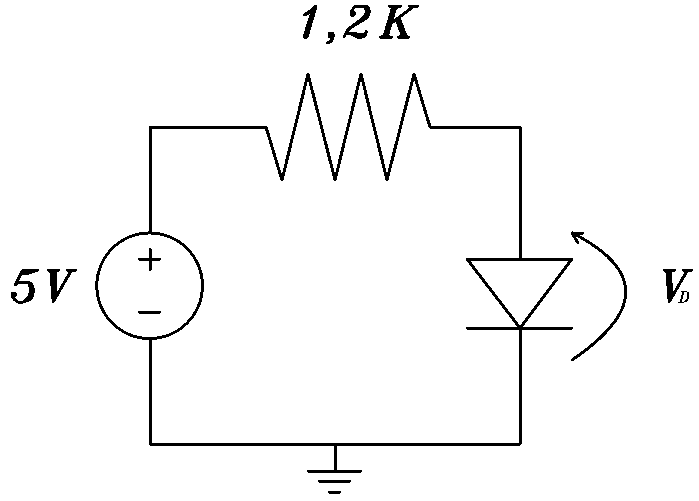
\includegraphics[width=0.6\linewidth]{resources/circuito_diodo_5v.png}
\caption{Esquema del circuito}
\label{fig:circuito_diodo_5v}
\end{minipage}
\begin{minipage}{.5\textwidth}
\centering
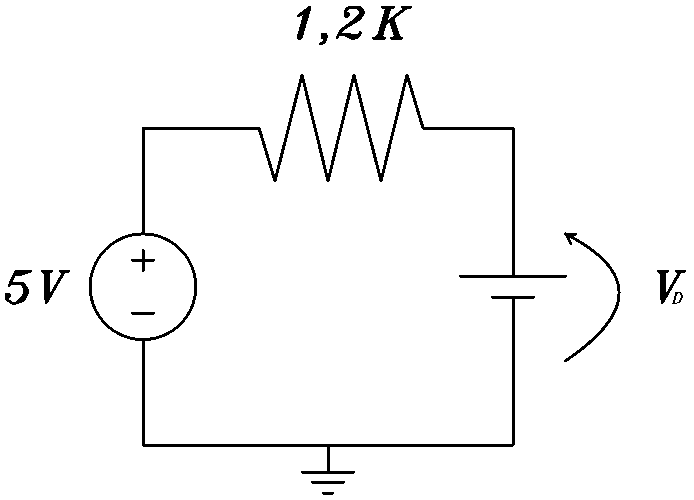
\includegraphics[width=0.6\linewidth]{resources/circuito_diodo_5v_simplificado.png}
\caption{Esquema del circuito simplificado}
\label{fig:circuito_diodo_5v_simplificado}
\end{minipage}
\end{figure}
\quad Para resolver el circuito de la Figura \ref{fig:circuito_diodo_5v} utilizando el modelo de orden cero, primero asumo que el diodo se encuentra en directa y lo reemplazo en el circuito por una caída de tensión de valor $V_D = 0,7V$, como se observa en la figura \ref{fig:circuito_diodo_5v_simplificado}.
\quad Luego, planteando ley de mallas en el circuito simplificado, tomando la dirección positiva de la corriente en sentido horario y despejando a esta misma, obtengo 
$$5V-I\times1,2K\Omega-V_D=0 \implies I=\frac{5V-V_D}{1,2K\Omega}$$ Finalmente, reemplazando $V_D$ con el valor supuesto por el modelo, se obtiene $I = 3,583mA$. Como la dirección positiva de corriente elegida coincide con la dirección esperada para un diodo en directa en la configuración de el circuito de la figura \ref{fig:circuito_diodo_5v}, se considera la asunción inicial de el estado del diodo correcta.
\subsection{Caso $V_s = -5V$}
\begin{figure}[ht!]
\begin{minipage}{.5\textwidth}
\centering
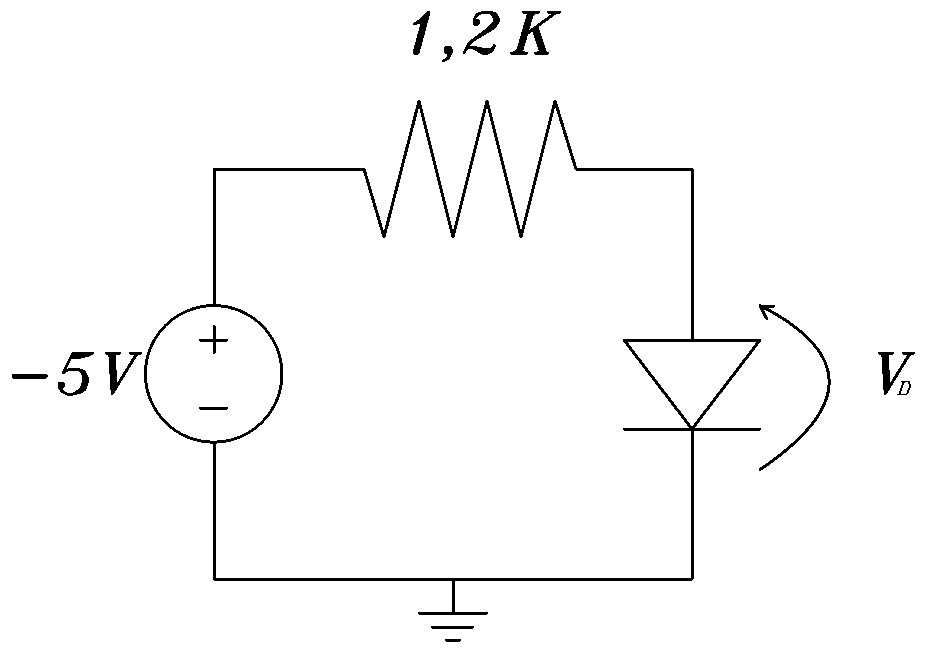
\includegraphics[width=0.6\linewidth]{resources/circuito_diodo_-5v.png}
\caption{Esquema del circuito}
\label{fig:circuito_diodo_-5v}
\end{minipage}
\begin{minipage}{.5\textwidth}
\centering
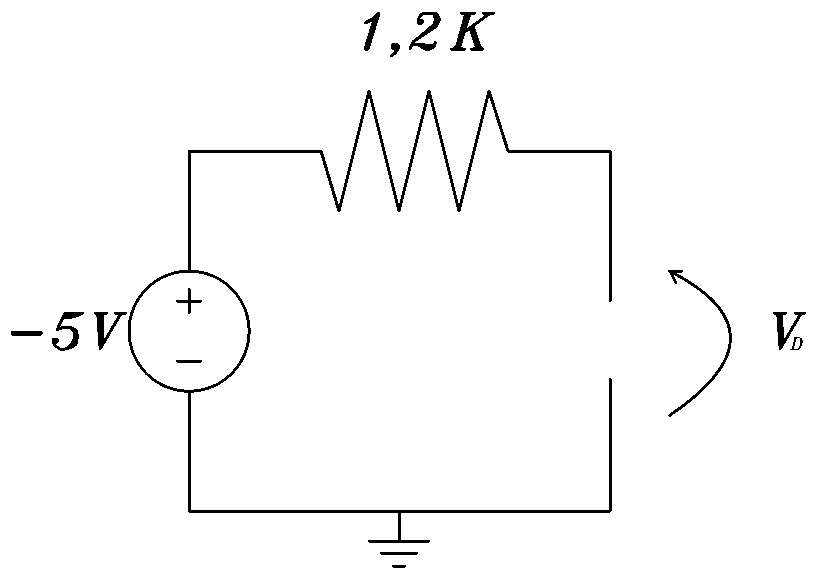
\includegraphics[width=0.6\linewidth]{resources/circuito_diodo_-5v_simplificado.png}
\caption{Esquema del circuito simplificado}
\label{fig:circuito_diodo_-5v_simplificado}
\end{minipage}
\end{figure}
\quad Para el circuito de la figura \ref{fig:circuito_diodo_-5v}, asumo inversa y reemplazo por su equivalente en el modelo, que en este caso es un circuito abierto, como se puede observar en la figura \ref{fig:circuito_diodo_-5v_simplificado}. Al estar la malla abierta, no circula corriente, por lo que $V_D$ resulta igual a la tensión de la fuente, $-5V$. Esto implica que la asunción de el estado del diodo es correcta.

%-----------------------------------------------------------------------------------------------
\section{Simulación de la característica I-V y extracción de parámetros}
\quad Para obtener los parámetros necesarios para utilizar el modelo exponencial del diodo primero simulé el circuito de la figura \ref{fig:circuito_simulacion_spice} en el modo barrido DC entre -0,8V y 0,8V con el objetivo de obtener la curva de relación tensión-corriente.

\begin{figure}[ht!]
    \centering
    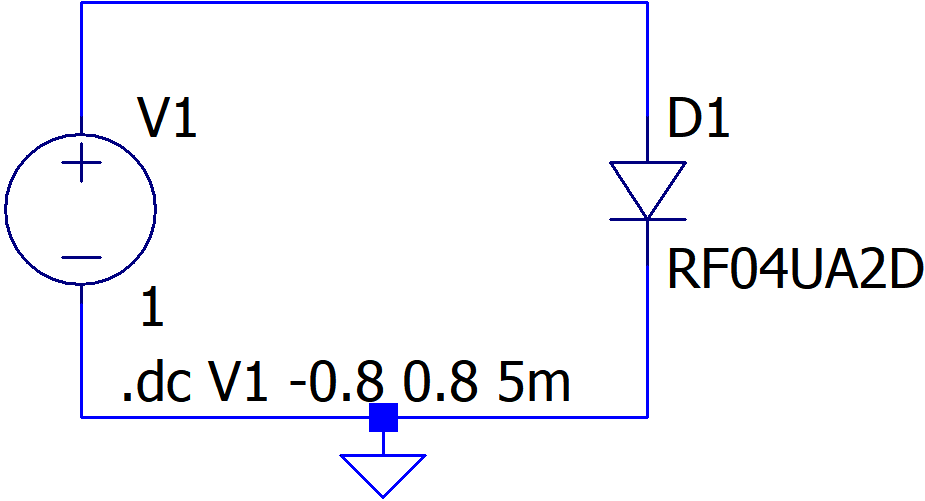
\includegraphics[width=0.4\linewidth]{resources/circuito_simulacion_spice.png}
    \caption{Circuito a simular en LTspice}
    \label{fig:circuito_simulacion_spice}
\end{figure}

\quad Luego, utilizando el script provisto por los profesores, y el programa Octave obtuve gráficos de la curva tensión-corriente en escala lineal (figura \ref{fig:grafico_escala_lineal}) y escala logarítmica (figura \ref{fig:grafico_escala_logaritmica}),y luego de ajustar la curva en escala semilogarítmica con los valores de tensión entre 200mV y 600mV obtuve valores para el factor de idealidad (n=1,198) y la corriente de saturación inversa ($I_s = 5,640pA$)

\begin{figure}[ht!]
\begin{minipage}{.5\textwidth}
\centering
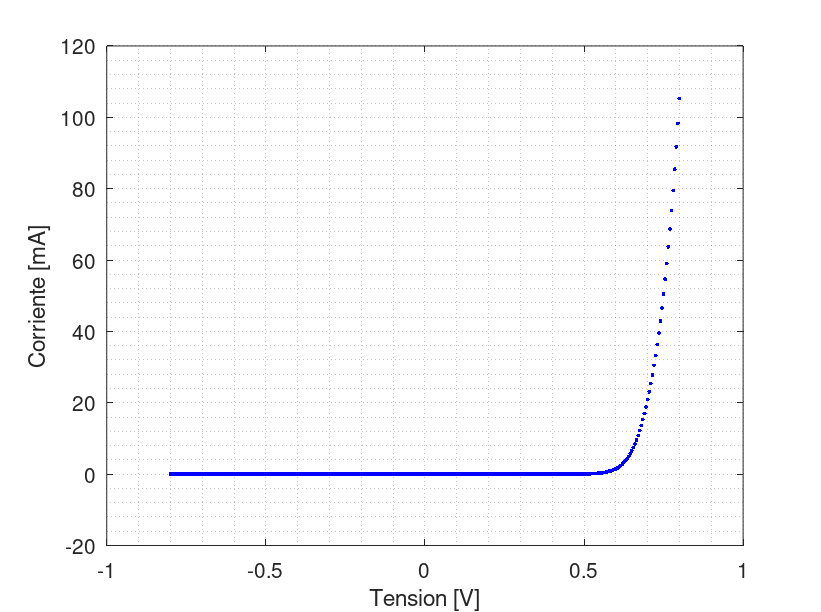
\includegraphics[width=1.1\linewidth]{resources/grafico_escala_lineal.png}
\caption{Gráfico en escala lineal}
\label{fig:grafico_escala_lineal}
\end{minipage}
\begin{minipage}{.5\textwidth}
\centering
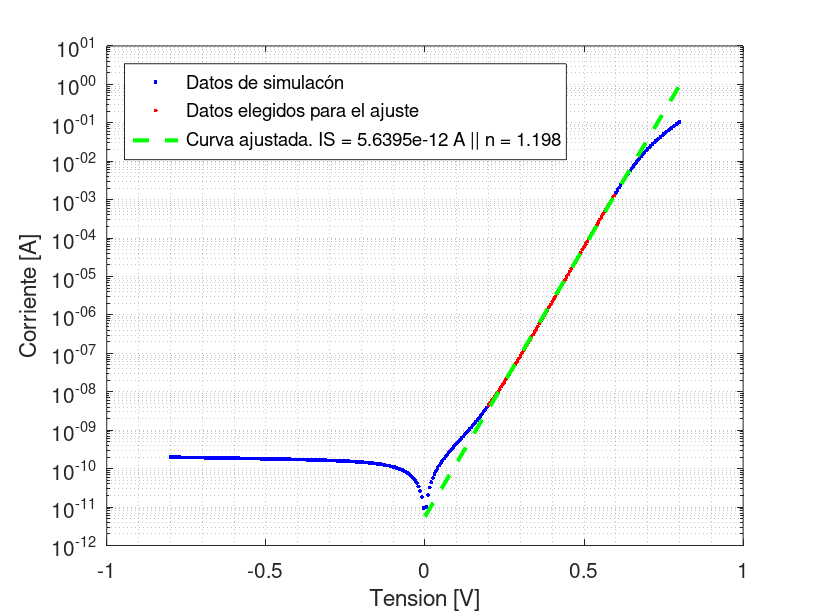
\includegraphics[width=1.1\linewidth]{resources/grafico_escala_logaritmica.png}
\caption{Gráfico en escala logarítmica con curva ajustada}
\label{fig:grafico_escala_logaritmica}
\end{minipage}
\end{figure}

%-----------------------------------------------------------------------------------------------
\section{Resolución del circuito con modelo exponencial}
\quad El modelo exponencial es uno de los mas precisos a la hora de modelar la relación tensión-corriente a través de un diodo. Éste se basa en la ecuación $$I_D = I_s(e^{\frac{V_D}{nV_{th}}}-1)$$ Donde $V_{th}$ es el potencial térmico, viene dado por $V_{th} = \frac{kT}{q}$ y para las cuentas de este informe se considera la temperatura constante y $V_{th}$ = 25,8mV. $I_s$ y n son constantes que dependen de los parámetros físicos del diodo, y para el caso a analizar fueron obtenidos en el inciso anterior.
\subsection{Caso $V_s = 5V$}
Planteando ley de mallas en el circuito de la figura \ref{fig:circuito_diodo_5v} y despejando la corriente se obtiene $$5V - V_D -I_D\times1,2K = 0 \implies I_D = \frac{V_S-V_D}{1,2K}$$
Luego, despejando $V_D$ en la ecuación exponencial del diodo (despreciando el -1, ya que $V_d > 5V_{th}$) $$V_D = n\times V_{th}\times Ln(\frac{I_D}{I_s})$$
Como el sistema caracterizado por las ecuaciones anteriores no tiene solución analítica, utilizo un método iterativo iniciando con $V_D = 500mV$ e $I_D = 3,75mA$. Luego de 3 iteraciones, se concluye que $V_D = 627mV$ e $I_D = 3,644mA$.
\subsection{Caso $V_s = -5V$}
\quad Luego de un rápido análisis del circuito de la figura \ref{fig:circuito_diodo_-5v} resulta evidente que el diodo está en estado de inversa (corroborado en sección 1.2). También, analizando la ecuación exponencial dada más arriba (esta vez sin despreciar el -1, ya que no se cumple la condición anterior), se puede apreciar que cuando $V_D$ es negativo, y mayor en módulo que $V_{th}$ (en el curso se toma $|V_D|>5V_{th}$) el termino con la exponencial se aproxima a cero y toda la expresión se aproxima a $-I_S$. Por esto, se considera que para este caso $I_D = 5,640pA$ y $V_D = -5V$

%-----------------------------------------------------------------------------------------------
\section{Resultados y análisis}
\quad Iniciando con el análisis de los gráficos con el de la figura \ref{fig:grafico_escala_logaritmica}, se puede apreciar a simple vista que ocurre un desvío aproximándose a los 800mV entre la curva simulada por LTspice y la ajustada. Más precisamente, a los 800mV se puede apreciar un error relativo de 7,8 en la curva ajustada respecto a la simulada, lo cual puede resultar contraproducente en situaciones próximas a este valor. Sin embargo, para tensiones entre 200mV y 600mV el error es indistinguible por lo que el modelo exponencial resulta una aproximación viable.

\quad Luego, comparando los resultados obtenidos al resolver los circuitos de las figuras \ref{fig:circuito_diodo_5v} y \ref{fig:circuito_diodo_-5v} mediante ambos modelos, como se puede ver en el cuadro \ref{tab:cuadro_comparativo_de_resultados}, en el caso de 5V, el error de la corriente del modelo de orden cero con respecto al exponencial es mucho menor que el error de la tensión. En el caso de -5V el error de la corriente del modelo de orden cero es mucho mayor, pero en este caso, el error absoluto es muy pequeño, por lo que puede ser util para ciertas aplicaciones
\begin{table}[ht!]
  \begin{center}
    \caption{Resultados obtenidos al resolver utilizando los distintos modelos}
    \label{tab:cuadro_comparativo_de_resultados}  %etiqueta para referenciar la tabla
    \begin{tabular}{|l|l|l|l|} % cantidad de columnas que va a tener representadas por las letras l, c, r, que indican el alineamiento (left, center, right). Una barra vertical "|" entre dos letras representa una linea dibujada entre las dos columnas
    \hline
      Parámetro & Orden 0 & Exponencial & Error relativo\\ 
      \hline
      $V_D(5V)$ & 700mV & 627mV & 0,12\\
      \hline        %este comando entre dos filas, agrega una línea que las separa
      $I_D(5V)$ & 3,583mA & 3,644mA & 0,02\\
      \hline
      $V_D(-5V)$ & -5V & -5V & 0\\ 
      \hline
      $I_D(-5V)$ & 0 & 5,640pA & 1\\
      \hline
    \end{tabular}
  \end{center}
  
\end{table}


%-----------------------------------------------------------------------------------------------
\section{Conclusiones}
\quad Los resultados obtenidos se encuentran dentro de lo esperado, en el caso de la resolución del circuito, los resultados obtenidos mediante los dos modelos son comparables, por lo que ambos modelos pueden resultar útiles para ciertas circunstancias. El modelo exponencial resulta más fiel al modelo simulado, sin embargo el error se vuelve significativo a la hora de aproximar la corriente por fuera del intervalo mencionado en el inciso 4. El modelo de orden 0, si bien difiere significativamente de la simulación, resulta útil para algunos análisis más rápidos, como bien pueden ser los que se realizan en etapas iniciales del diseño de circuitos, donde las características especificas del diodo a utilizar pueden no conocerse.

\quad El trabajo resultó útil para afianzar los conocimientos de las características eléctricas de los diodos de juntura, sin embargo, el máximo de hojas resulta limitante, ya que, de haber podido, hubiera incluido mayor detalle en cada uno de los incisos.

%-----------------------------------------------------------------------------------------------




\end{document}
